\subsection{Basics of Electronics}

In this section, we'll have a look at fundamental concepts in electronics.  We'll also point you to the right references to understand the concept if our explanations are not enough. I believe the best way to grasp these challenging concepts is through water analogies: as we see water every day (as opposed to electrons), it is a lot easier to understand elementary fluid dynamics concepts than elementary electricity concepts. Fortunately, whoever created this world loved the concept of \textit{Fractals} and self-similar patterns, so it's very easy \footnote{Honestly it's almost scary how similar it is, you'd believe it's all the same thing. This makes me thing of a slightly unrelated essay which thinks about a somewhat related epistemological problem: \url{https://en.wikipedia.org/wiki/The_Unreasonable\_Effectiveness\_of\_Mathematics\_in\_the\_Natural\_Sciences}} to make accurate electricity analogies with fluids.  
Because this course goes in depth into electronics, it is assumed that all these concepts are already fairly familiar to the student. We have chosen to cover it just as a reminder or merely a pointer to what one should know before starting the course. If one is not fully comfortably with these concepts, time should \textit{first} be spent understanding them before going further into the course. It is not needed to enter into deep theory, but one should be comfortable enough with the conceptual behaviour in order to understand the rest of the course. 

\subsubsection{Fluid Model: The Key to Understanding Electronics.}

This section is largely inspired by Carver Mead's \textit{Analog VLSI} textbook, which I cannot recommend enough. 

\begin{figure}[H]
    \centering
    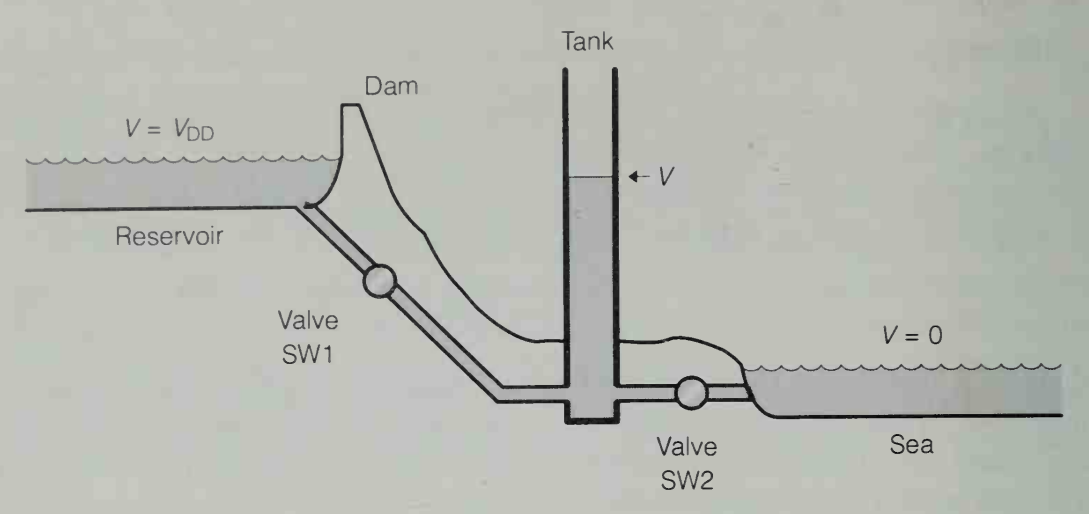
\includegraphics[width=0.65\linewidth]{../../Figures/Water_Analogies_Carver_Mead.PNG}
    \caption{Hydraulic analogy of electronic (or neural) circuit. The power supply is a reservoir of water at potention $V_{dd}$. The reference potential is sea level, corresponding to \textit{ground} of electrical circuits. The water level in the tank corresponds to the output voltage. The tank can be filled by opening the valve SW1 or emptied by opening valve SW2 - the valves can be compared to switches in electrical circuit. Adapted from Carver Mead \textit{Analog VLSI} textbook}
    \label{fig:Hydraulic Anlogy}
\end{figure}

We are able to use fluid analogies to describe electrical dynamics because the fundamental component of electrical circuit (the charged particle - be it ions or electrons) is present in sufficient number that they cannot be accounted for individually - similarly to fluid dynamics where we cannot model at the scale of the individual fluid molecule. The quantity of water in figure \ref{fig:Hydraulic Anlogy} is analogous to the quantity of electrical charge $Q$. There is an underlying granularity to these quantities: water is made up of water molecules, charge in a neuron is made up of ions (more on that later) and charge in a transistor is made up of electrons. In all cases, we can discuss the quantity in terms of either the number of elementary particles or a more convenient macroscopic unit.  

In electronics, the flow of the fundamental particle is called the \textbf{electrical current}. When speaking of fluids dynamics, gravity is a critical force that will impact much of the behaviour of this fluid - in electronics, the analogous gravitational "potential" is called \textbf{voltage}. In figure \ref{fig:Hydraulic Anlogy}, it corresponds to the height at which the water stands compared to the reference point: sea level. It is quite straightforward to understand from this point of view that, exactly as the water which is up in the reservoir is drawn to the ground (but doesn't necessarily reach if the valves are closed), electrical charge at a given potential is attracted to the electrical ground (but doesn't necessarily reach if switches are "opened" i.e. not allowing electrons to flow). This is what potential difference/voltage represents. This leads to the following observation, which makes up for most of what needs to be understood about fundamental electricity behaviour: a \textit{potential difference} in charge drives a \textit{current flow} from a higher potential point to a lower potential point, and it flows relative to the extent by which we let it flow: how \textit{conductive} (or resistive) the path between the high and low potential points is. This is what makes up for Ohm's law, where Current = Potential Difference / Resistance - we'll get to this again later. Resistance/Conductivity in this analogy corresponds to the diameter and material used in the pipes linking the reservoir to the sea - the larger the diameter and the smoother the material of the piper, the easier water can flow, the opposite also holds. 

It is interesting to note that we can measure the height of water from any reference point we choose. There is however one particular advantage to choosing "sea level" as the reference potential: the height will always be positive or zero, thereby making calculations easier. In electrical circuits, this point of reference is called ground, and it is at 0 Volts. 

You might wonder what happens when we run out of water in the reservoir. In fluid dynamics we'd need a pump (and thus some energy) to bring back water to the top. This is somewhat similar in electrical systems, which typically use an electrochemical process (such as in batteries) to keep on bringing electrical charge into the "reservoir".\footnote{There are obviously many other processes to keep the level of charge in the reservoir to a certain level, but no need to get into that. Just know that it doesn't get there magically, energy is needed to get it there. This is why batteries run out, or why you don't have electricity in your house if you don't pay your electricity bill - in both cases, the supply of charge in the reservoir stops.}  

Now that this has been introduced, we can look in a bit more details into each of the concepts that should be understood, and keep on going back to water analogies to make things clear. Let's start with the fundamental electrical component: electrical charge. 

\subsubsection{Charge}

This is the water molecule in the hydraulic analogy: the fundamental component which behaviour we describe. In fact, we never really describe the behaviour of the individual component, but rather the behaviour of the aggregate of individual components. 
Electric charge is the physical property of matter that causes it to experience a force when placed in an electromagnetic field. Think of a charge in an electromagnetic field as you think of some matter in a gravitational field - it is subject to forces because it has a mass. Electrical charge is subject to a force because it is not "neutral". 
Electric charge can be positive or negative (commonly carried by protons and electrons respectively). A somewhat fundamental electrical charge can also be an ion rather than electron or proton. An ion is an atom which has lost or gained one electron through some chemical process - as it has lost a charged particle, it therefore becomes charged itself, either positively or negatively. Alike charges repel each other and unlike charges attract each other. An object with an absence of net charge is referred to as neutral. We define charge with the symbol $Q$ and with the units of \textit{Coulombs}. An electron has, by convention, a charge of $1.6 \cdot 10^{-19}$ Coulombs.  

\subsubsection{Electric Field}

An electric field is the physical field that surrounds electrically-charged particles and exerts force on all other charged particles in the field, either attracting or repelling them. By convention, the electric field vector \vec{E} points from positive to negative. Electric field also refers to the physical field for a system of charged particles. It's conceptually a bit similar to Newton's gravitational law, where all matter possessing a mass exerts a force on other masses, depending on the distance that separates them (and the Gravitational Constant). Understanding electric field is important to understand the physics behind transistors, and it actually is not so obvious to grasp. It would take me quite some time to explain it well, as it is not a concept that the water analogy can explain easily - I thus recommend having a look at the \textit{Khan Academy} \footnote{https://www.khanacademy.org/science/hs-physics/x215e29cb31244fa1:types-of-interactions/x215e29cb31244fa1:electric-and-magnetic-fields/v/electric-field-definition} explanation as I won't be able to do anything better than this. 

\subsubsection{Voltage}

Voltage\footnote{Section mostly copy-pasted from: https://www.electronics-tutorials.ws/dccircuits/dcp\_1.html}, ($V$) is the potential energy of an electrical supply stored in the form of an electrical charge. Voltage can be thought of as the force that pushes electrons through a conductor and the greater the voltage the greater is its ability to “push” the electrons through a given circuit. The difference in voltage between any two points, connections or junctions (called nodes) in a circuit is known as the Potential Difference, (p.d.) also commonly called the Voltage Drop. The Potential difference between two points is measured in Volts with the circuit symbol V, or lowercase “v“.

\textbf{Voltage is always measured as the difference between any two points in a circuit and the voltage between these two points is generally referred to as the “Voltage drop“}. Note that voltage can exist across a circuit without current, but current cannot exist without voltage and as such any voltage source whether. This makes sense in the hydraulic analogy - there can be a height difference but no water flowing but there cannot be a flow without height difference \footnote{Yes, yes, I know, you can have water flowing in a flat surface but this is either because you push it somehow or because there is height drop somewhere further - in any case, water always flows as a result of some force being applied, either gravity or something human generated.}. 

\begin{figure}[H]
    \centering
    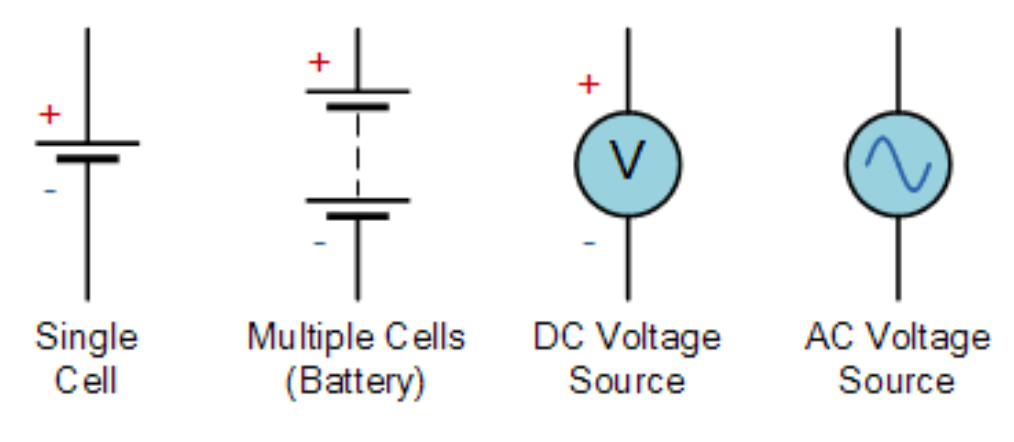
\includegraphics[width=0.65\linewidth]{../../Figures/Voltage.PNG}
    \caption{Voltage symbol. Adapted from https://www.electronics-tutorials.ws/dccircuits/dcp\_1.html}
    \label{fig:Resistors}
\end{figure}

\subsubsection{Current}

Electrical Current \footnote{Section mostly copy-pasted from: https://www.electronics-tutorials.ws/dccircuits/dcp\_1.html} ($I$), is the movement or flow of electrical charge (most usually electrons) and is measured in Amperes, symbol I (or i), for "intensity". It is the continuous and uniform flow (called a drift) of charge around a circuit that are being “pushed” by the voltage source (height difference). In reality, electrons flow from the negative terminal to the positive terminal of the supply (as electrons are negative and thus attracted by positive point); however, for ease of circuit understanding conventional current flow assumes that the current flows from the positive to the negative terminal.
This is why, by convention, the flow of current in circuit diagrams is represented by an arrow pointing from the positive to the negative node, despite electrons flowing from negative to positive node. This convention goes back to Benjamin Franklin: \textit{"As far as the history goes, Ben Franklin imagined electricity as a type of invisible fluid that could build up or be absent from a material, or at least certain materials. He believed that when this invisible fluid built up the object was positively charged. When there was an absence of this fluid he called that material negatively charged. It turns out he got the concept right but the nomenclature backwards."}. So it really is because of him that conventional current flow is not in the same direction as electron flow. Once you get used to it, it's fine, but this can be quite annoying sometimes when you're trying to visualize how circuits work. 

\begin{figure}[H]
    \centering
    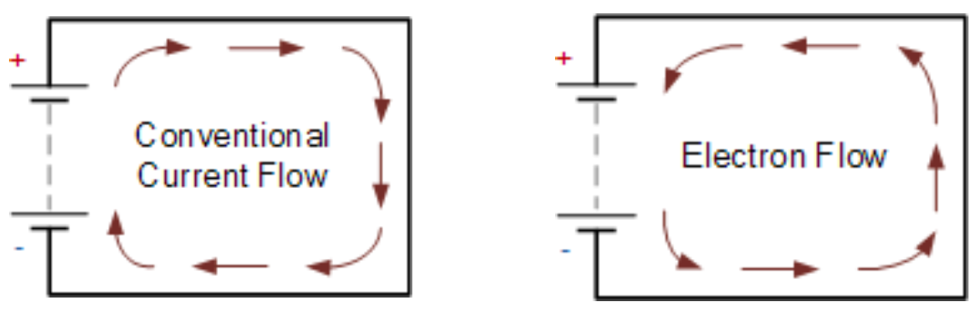
\includegraphics[width=0.85\linewidth]{../../Figures/Electron_Flow.PNG}
    \caption{Electron flow and conventional current. Adapted from https://www.electronics-tutorials.ws/dccircuits/dcp\_1.html}
    \label{fig:Resistors}
\end{figure}

Current is defined by the following important relation: 

\begin{equation}
    I = \frac{dQ}{dt}
\end{equation}

This becomes very clear in the hydraulic analogy, as we quantify the flow of water by the quantity of water flowing at a given point in time. 

\subsubsection{Resistance}

\begin{figure}[H]
    \centering
    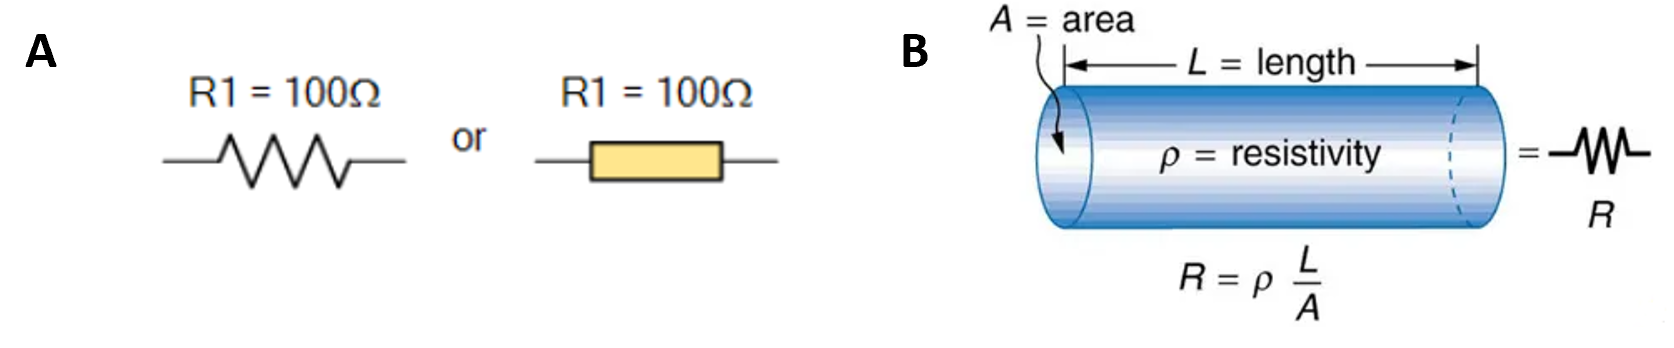
\includegraphics[width=0.65\linewidth]{../../Figures/Resistors.PNG}
    \caption{Resistor electric symbols. Adapted from https://www.electronics-tutorials.ws/resistor/res\_1.html}
    \label{fig:Resistors}
\end{figure}

In the hydraulic analogy figure \ref{fig:Hydraulic Anlogy}, if both valves \footnote{keep in mind from the first section that valves are simply switches, allowing water (or current) to flow (or not). They can be thought of elements with infinite resistance when blocking flow, and 0 resistance when allowing flow} are opened, water will flow from the reservoir into the sea at a finite rate, restricted by the diameter of the pipe through which it must flow. If the water level in the reservoir is increased, water will flow more quickly (up to a certain level), and the inverse is also true. The property of the pipe diameter and material, which restrict the flow of water, is called resistance. The electrical element possessing this quality is called a resistor. 

The principal job of a resistor within an electrical circuit is thus to “resist” (hence the name Resistor), regulate or to set the flow of electrons (current) through them by using the type of conductive material from which they are composed. Resistors can also be connected together in various series and parallel combinations to form resistor networks which can act as voltage droppers, voltage dividers or current limiters within a circuit. This is analogous to separating an original pipe into multiple pipes where flow divides.  

It is important to note that current is not affected by resistance in a \textit{closed loop} circuit, because there is always \textbf{the same quantity of charge flowing in the loop}. In other words, current is constant everywhere in the closed loop circuit (admitting we do not add new elements), as long as there is current flowing.  Voltage however, drops when encountering the different valves, simply because the height difference is reduced throughout water descent. This can seem a bit counterintuitve, but it will become clearer as we go through series and parallel circuits later.  

Resistors are represented in electrical circuits as shown in figure \ref{fig:Resistors}. A and resistance is measured in \textit{Ohms} ($\ohm$). They are called “Passive Devices”, because they contain no source of power or amplification but only attenuate or reduce the voltage or current signal passing through them. This attenuation results in electrical energy being lost in the form of heat as the resistor resists the flow of electrons through it.

Most types of resistor are linear devices that produce a \textit{voltage drop} across themselves when an electrical current flows through them. Different values of resistance produces different values of current or voltage. This can be very useful in Electronic circuits by controlling or reducing either the current flow or voltage produced across them we can produce a voltage-to-current and current-to-voltage converter.

The resistance of any substance depends on the following factors: 1) the length of the device ($L$), 2) the cross sectional area of the device ($A$), 3) the nature of material of the device, which has an inherent \textit{resistivity} ($\rho$, measured in $\ohm.m$), 4) the temperature of the device ($T$) (see Figure \ref{fig:Resistors}.B). All these variables also apply to evaluate pipes resistance in the water analogy! 

\begin{equation}
    R = \rho \frac{L}{A}
\end{equation}

We say that a physical element or device has \textbf{infinite resistance} when current doesn't flow through it: it is an \textbf{insulator}. In practice, there is always a tiny tiny bit of current flowing, simply because infinite resistance is not realistic. To understand properly why this is the case, we would need to look into the physics of conduction, which will be covered in chapter 2 when introducing the transistor physics. For now, just imagine a big big wall - as big and strong as it is, if you have a strong enough water pressure applied on it, it may eventually break and allow current to pass. Another thing is that, even if it doesn't break, the wall cannot prevent water molecules which evaporate to pass to the other side. Moral of the story, even with very high resistance, you always have some flow, and there is no such thing as absolutely infinite resistance - it can always break. And exactly like in the water analogy, resistors can break if we apply too strong of an energy on them. 

One last thing, it is often convenient to view an electrical circuit element in terms of its \textit{willingness} to carry current rather than its reluctance to do so. As such, we often speak of \textit{conductance} rather than resistance. Both properties are analogous and represent essentially the same idea. Conductance, represented with the letter $G$ (sometimes $g$) is simply the inverse of resistance: $G = \frac{1}{R}$

\subsubsection{Ohm's law}

Simply, there is a linear relationship that relates Voltage and Current: 
\begin{equation}
    I = \frac{V}{R} = V\cdot G
\end{equation}

A voltage of $1 Volt$ across a resistance of $1 \ohm$ will cause a current flow of $1 amp$.

\subsubsection{Capacitance}

\begin{figure}[H]
    \centering
    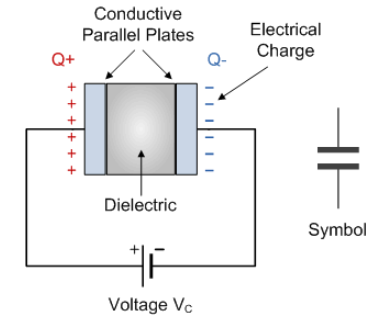
\includegraphics[width=0.55\linewidth]{../../Figures/Capacitors.PNG}
    \caption{Capacitor structure and electric symbol. Adapted from https://www.electronics-tutorials.ws/capacitor/cap_1.html}
    \label{fig:Capacitors}
\end{figure}

In the hydraulic analogy, the capacitor simply corresponds to the tank (with constant cross sectional area). Depending on cross sectional area, it will be able to hold a certain quantity of charge. It also needs time to charge up, and time to discharge. This leads to a shift in circuit analysis, where "steady state" analysis is not enough anymore - one must consider the charging and discharging properties of the capacitor as one would consider the flow relative to the the tank filling up and emptying itself. 

In its basic form, an electrical capacitor consists of two or more parallel conductive (metal) plates which are not connected or touching each other, but are electrically separated either by air or by some form of a good insulating material such as waxed paper, mica, ceramic, plastic or some form of a liquid gel as used in electrolytic capacitors. The insulating layer between a capacitors plates is commonly called the Dielectric.

Due to this insulating layer, current does not flow through the capacitor as it blocks it allowing instead a voltage to be present across the plates in the form of an electrical charge.

Also, because capacitors store the energy of the electrons in the form of an electrical charge on the plates the larger the plates and/or smaller their separation the greater will be the charge that the capacitor holds for any given voltage across its plates. In other words, larger plates, smaller distance, more capacitance. This yields the following relation:

\begin{equation}
    C = \frac{\epsilon_0 A}{d}
\end{equation}

with $C$ capacitance in Farads ($F$), $\epsilon$ permittivity of the dielectric \footnote{Permittivity is a measure of the electric \textit{polarizability} of a dielectric. A material with high permittivity polarizes more in response to an applied electric field than a material with low permittivity, thereby storing more energy in the material}, $A$ area of the plate overlap in $m^2$ and $d$ distance between the plates in meter. 

The capacitor is thus a component which has the ability or “capacity” to store energy in the form of an electrical charge producing a potential difference (Static Voltage) across its plates, much like a small rechargeable battery.
Capacitance is the electrical property of a capacitor and is the measure of a capacitors ability to store an electrical charge onto its two plates with the unit of capacitance being the Farad (abbreviated to F) named after the British physicist Michael Faraday

By applying a voltage to a capacitor and measuring the charge on the plates, the ratio of the charge Q (in Coulomns) to the voltage V (in Volts) will give the capacitance value of the capacitor and is therefore given by the following important relation: 
\begin{equation*}
    C = \frac{Q}{V}
\end{equation*}

One will then notice that $1 Farad = 1 Coulomb per Volt$

Although the charge is stored on the plates of a capacitor, it is more exact to say that the energy within the charge is stored in an “electrostatic field” between the two plates. When an electric current flows into the capacitor, it charges up, so the electrostatic field becomes much stronger as it stores more energy between the plates. Likewise, as the current flowing out of the capacitor, discharging it, the potential difference between the two plates decreases and the electrostatic field decreases as the energy moves out of the plates.

\textbf{Still not sure you understand?} If you feel like you still need to grasp the fundamental idea behind a capacitor, go watch the brilliant video by \textit{The Engineering Mindset} on capacitors \footnote{https://www.youtube.com/watch?v=X4EUwTwZ110}.

\subsubsection{DC vs AC and exponential notation}

The explanations dealt with so far have constant voltage sources and are just taken at "steady state" - think constant flow due to constant supply of water in the reservoir. Direct current (DC) is the flow of electric charge in a constant fashion. It is the steady state of a constant-voltage circuit. Most well-known applications, however, use a time-varying voltage source, yielding a time varying current, and time varying signals in general. This is relevant here not because we consider AC per se but rather because AC is a generalization of DC, and in some cases we need the time component (specifically with circuits with some capacitance). It is thus useful to be familiar with this concept, and most importantly, its notation. Alternating current (AC) is the flow of electric charge that periodically reverses direction. If the source varies periodically, particularly sinusoidally, the circuit is known as an alternating current circuit. Though batteries or power supplies are mostly used to produce a steady D.C. voltage source, A.C. (alternating current) voltage sources are used for domestic house and industrial power. This is for efficiency and transmission purposes, that we will not get into.

Figure 1 shows graphs of voltage and current versus time for typical DC and AC power. The AC voltages and frequencies commonly used in homes and businesses vary around the world. 

\begin{figure}[H]
    \centering
    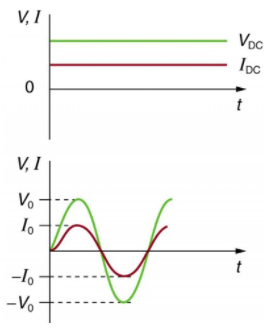
\includegraphics[width=0.35\linewidth]{../../Figures/ACDC.PNG}
    \caption{Alternating and direct current. Adapted from \url{https://courses.lumenlearning.com/physics/chapter/20-5-alternating-current-versus-direct-current/}}
    \label{fig:ACDC}
\end{figure}

If we're dealing with a different type of signal, we must use a different type of notation and consider the differences with DC. As can be seen on Figure \ref{fig:ACDC}, AC behaves in waves, so it is appropriate to treat is as such and use relevant notation that describes it properly. Also, we will be using conventional notation for time varying voltage $u(t)$ and current $i(t)$ (as opposed to V and I that were previously used). We can now define \footnote{I am here assuming that you are familiar with exponential notation of periodic signals. If you aren't I suggest you spend some time reviewing this.}:  

\begin{equation}
    u(t) = U\mathrm{cos}(\omega t + \phi) = Ue^{j\omega t + \phi}\footnote{This is derived from Euler's formula: $e^{jx} = \mathrm{cos}(x) + j\mathrm{sin}(x)$}
\end{equation}

Where $U$ is the amplitude (peak value) of voltage, $\omega$ is the angular frequency, $\phi$ is the phase offset (more on the phase in a second).

\paragraph{Impedance}

There is a generalization of resistance, called \textit{impedance} (represented by the symbol $Z$). It is also measured in Ohms. It is not really useful when working with DC current, but takes meaning when working with AC current, which has a complex component to it (which we call reactance but we don't care about that). \textbf{Ohm's law still applies in AC} and impedance is simply the ratio of the complex wave representation of sinusoidal voltage ($u(t)$) between its terminals to the complex wave representation of the current ($i(t)$) flowing through it.  Impedance therefore possesses both magnitude and phase; resistance, on the other hand, has magnitude but no phase. This is why we say that impedance is a generalization of resistance, as resistance is only a special case of impedance. For impedance, we note: 

\begin{equation}
    Z = R + jX
\end{equation}

where R is the real part resistance and the imaginary part X is the reactance. The magnitude of $Z$ is $|Z| = \sqrt{R^2 + X^2}$, while the phase is $\phi = \mathrm{arctan}(\frac{X}{R})$. In general, $\phi$ is the phase difference between alternating voltage and current: $\phi = \phi_v - \phi_i$ 

\paragraph{Capacitance in complex analysis}
Capacitance is most often studied with complex analysis, so let's do that here and apply it to Ohm's law. While the current flowing through a resistor is given by the voltage applied to it, the current that flows through a capacitor is proportional to the voltage change. 

\begin{equation}
    i(t) = \frac{dQ}{dt} = \frac{d(C V)}{dt} = C\frac{du(t)}{dt}
\end{equation}

Here, $i(t)$ is the current through time, which we defined previously as being the derivative of charge Q with respect to time. We also previously defined Q as being equal to the capacitance times voltage V (following from $C = Q/V$). 

Differentiation can be conveniently performed in complex notation, yielding the following: 

\begin{equation}
    \frac{du(t)}{dt} = \frac{d (Ue^{j\omega t)}}{dt} = j\omega U e^{jwt} = j\omega u(t) 
\end{equation}

Therefore, for a capacitor, $i(t) = C\frac{du(t)}{dt} = j\omega \cdot C \cdot u(t)$

\subsubsection{Basics of Parallel and Series circuits}

\begin{figure}[H]
    \centering
    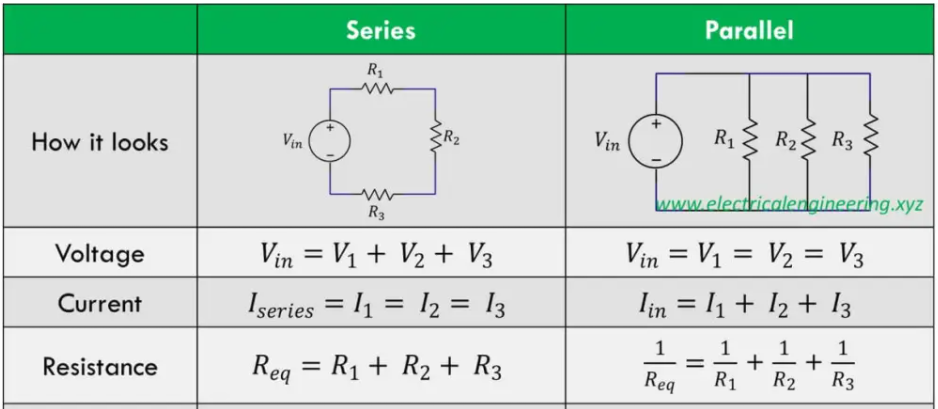
\includegraphics[width=0.75\linewidth]{../../Figures/Parallel_Series.PNG}
    \caption{Parallel and Series circuit comparison. Adapted from \url{https://www.electricalengineering.xyz/questions/top-5-differences-between-series-and-parallel-circuits/}}
    \label{fig:Parallel_Series}
\end{figure}

When dealing with electronic circuits, you can connect things in a variety of different ways, and some key things are to remember. Figure \ref{fig:Parallel_Series} does a great job at explaining this. Voltage drops across devices connected in series, but it is conserved across different branches of a circuit. Imagine having one branch separating into different branches on the same surface in the circuit: as all the pipes are at the same height from ground, they have the same voltage. Current is just the opposite, which make sense when you think of hydraulic analogy: it divides when separated into different branches and is maintained when flowing around a single loop. Resistance adds itself in series, which means that connecting two resistors together in the same branch makes the overall resistance stronger. This doesn't apply in parallel, where another relation need to be applied to find the total resistance of the circuit. If you have two branches and one has higher resistance than the other (pipe with small diameter), more current will flow through the lower resistance ones than the higher resistance one! 

Capacitance, which is not shown on the figure, is actually exactly the opposite of resistance, it adds up in parallel and follows the same principle as resistance in parallel when it is connected in series. 

\subsubsection{Kirchoff's Voltage and Current Laws}

One very important law is needed to understand many circuits we'll be studying: Kirchoff's voltage and current laws. 

\begin{itemize}
    \item Current law: All current flowing into a node (or junction) must be equal to the current flowing out of it. This means that there is no charge (think water) disappearing.
    \begin{equation}
        \sum I_{in} = \sum I_{out}
    \end{equation}
    \item Voltage law: In any complete loop within a circuit, the sum of all voltages across components which supply electrical energy (such as cells or generators) must equal the sum of all voltages across the other components in the same loop. This law is a consequence of both charge conservation and the conservation of energy. Think of a closed loop of reservoir at different height points which yield a continuous flow. Sum of heights will add up to 0.
    \begin{equation}
        \sum V_{total} = 0
    \end{equation}
\end{itemize}

The following figure\footnote{Adapted from: https://www.sciencefacts.net/kirchhoffs-law.html} makes this much easier to understand.  

\begin{figure}[H]
    \centering
    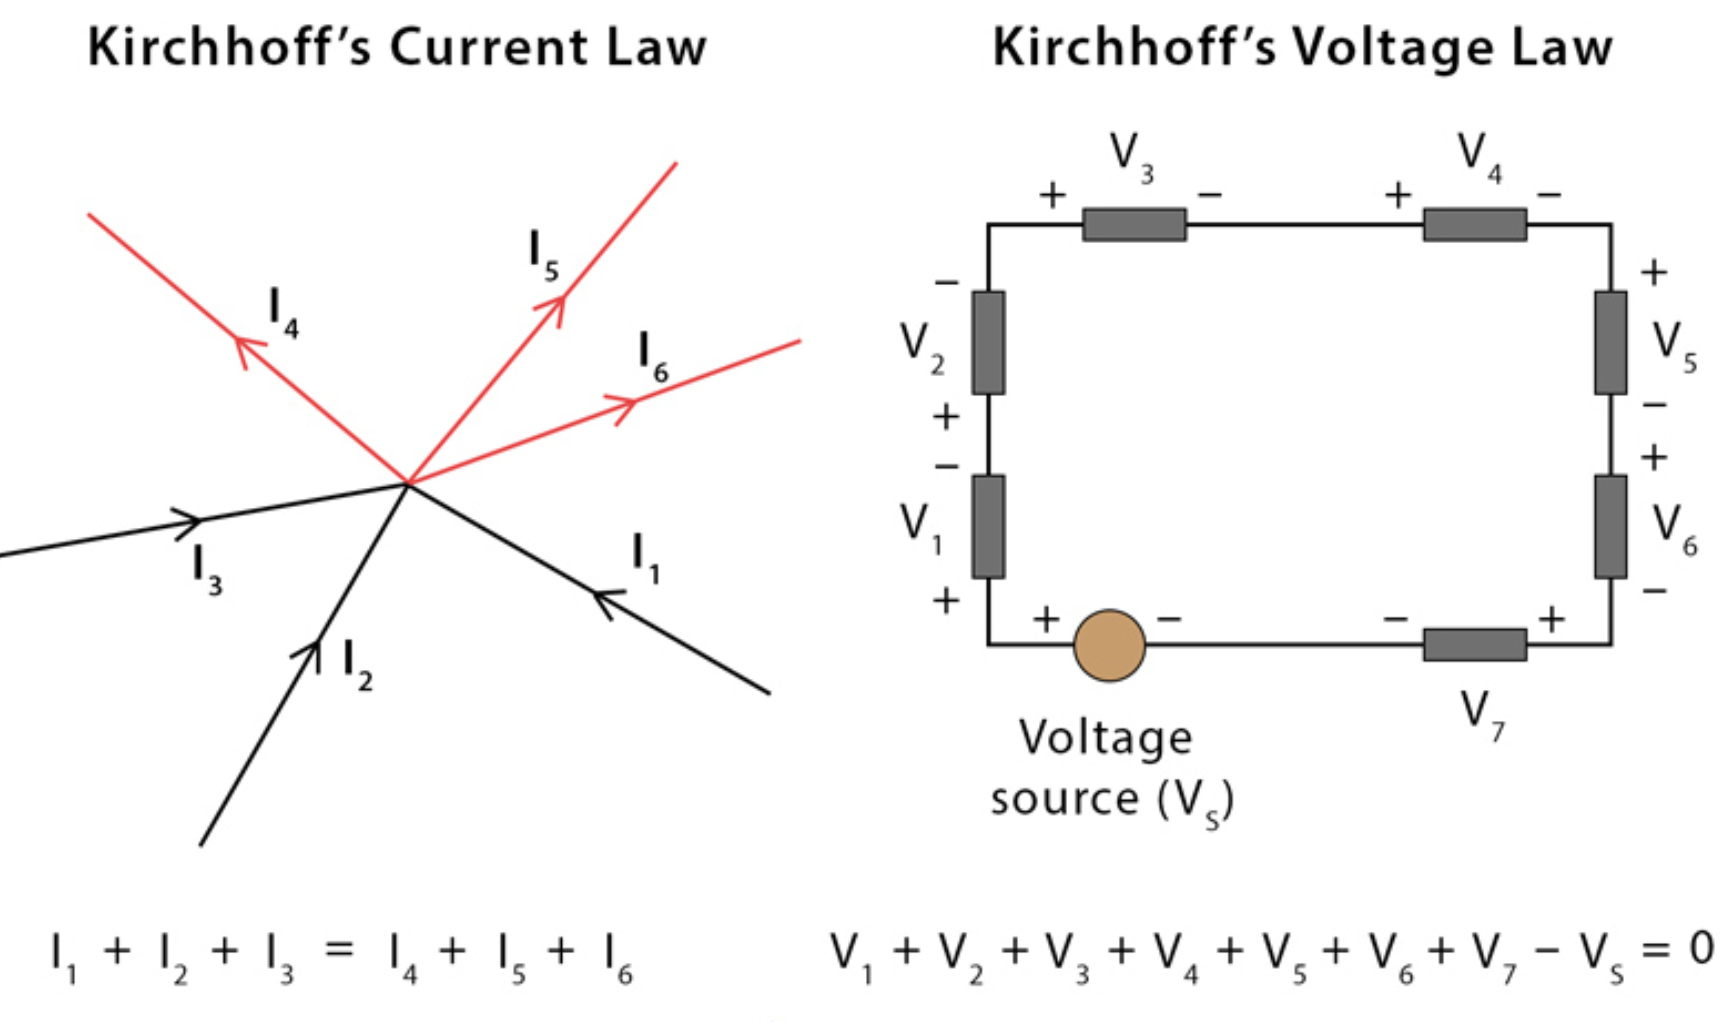
\includegraphics[width=0.7\linewidth]{../../Figures/Kirchoff.PNG}
    \caption{Kirchoff's current and voltage laws. Adapted from \url{https://www.electronics-tutorials.ws/capacitor/cap_1.html}}
    \label{fig:Capacitors}
\end{figure}

These are, I believe, all the necessary pre-requisites to understand the content of the module. Now we can build up from this and start understanding basics of transistors. But before heading there, let's look at some biology pre-requisites and try to explain them!


